\documentclass[11pt]{article} % The default font size and one-sided printing (no margin offsets)

\usepackage[square, numbers, comma, sort&compress]{natbib} % Use the natbib reference package - read up on this to edit the reference style; if you want text (e.g. Smith et al., 2012) for the in-text references (instead of numbers), remove 'numbers' 
%%%%%%%%%
\usepackage{amsmath,amsfonts,amsthm,amssymb}
\usepackage{setspace}
\usepackage{Tabbing}
\usepackage{fancyhdr}
\usepackage{lastpage}
\usepackage{extramarks}
\usepackage{chngpage}
\usepackage{soul,color}
\usepackage{graphicx,float,wrapfig}
\usepackage{times}
\usepackage{tabularx,ragged2e}
\usepackage{booktabs}
\usepackage{natbib}
\usepackage{epstopdf}
\usepackage{caption}
\usepackage{subcaption}
\usepackage[english]{babel}
\usepackage{lscape}
\usepackage{tikz}
\usepackage[linesnumbered,ruled,vlined]{algorithm2e}
\usepackage{multirow}
\usepackage{longtable}
\usepackage{array,booktabs}
%\usepackage{url}
\usepackage{hyperref}
%%%%%%%%%%
\hypersetup{urlcolor=blue, colorlinks=true} % Colors hyperlinks in blue - change to black if annoying
\title{\ttitle} % Defines the thesis title - don't touch this

\def\regmark{{\ooalign{\hfil\raise.07ex\hbox{\tiny R}\hfil\crcr
                    {\scriptsize\mathhexbox20D}}}}

\newcolumntype{P}[1]{>{\endgraf\vspace*{-\baselineskip}}p{#1}}
                    
\begin{document}
\renewcommand*{\arraystretch}{1.8}
\begin{titlepage}
\singlespacing
	\begin{center}
	\vspace*{1in}
	\begin{figure}
	\centering
	
\includegraphics[scale=0.5]{logo.jpg}
	\end{figure}
	\vspace*{0.1in}
	\LARGE \textbf{Work Progress Report}
	
	\vspace{0.2in}
	\large Project Period: 2015/02/16 $\sim$ 2015/08/18 \\
	\vspace{0.5in}
	{\Large \textbf{Praveenkumar VASUDEVAN}}
	\par
	\vspace{0.1in}
	\vspace{0.3in}
	\large Title\\
	\vspace{0.1in}
	\Large \textbf{Developing an experimental platform for Human Robot Interaction based on human motions}
	\end{center}
\end{titlepage}


\section{2015/02/15-2015/02/21}

\begin{center}
    \begin{longtable}{ | c | p{6cm} | p{5cm} |}
    \hline
    Date & Content & Problems/Remarks \\ 
    \endhead
    \hline

    2015/02/15         
    & 
    
    \begin{itemize}
      \item Arrival in Japan
    \end{itemize}
     &  - \\   		    
    \hline
                                          
    2015/02/16          
    & 
    \begin{itemize} 
    \item Project discussion with professor. 
    \item Showed demo of ALVAR toolkit, CMT (Consensus based matching and Tracking) toolkit. Demo based on PC webcam. 
    \item Received Kinect V2 sensor. 
    \end{itemize} 
  	&  - \\   		    
    \hline
  										 
    2015/02/17          
    & 
    \begin{itemize}
    \item Play with Kinect sensor SDK samples. 
    \item Setup Point cloud library environment. 
    \item Undergraduate presentation. 
    \item Welcome party.
    \end{itemize}   
    & 
    \begin{itemize}
    \item Problem with acquiring Kinect data and displaying in PCL viewer.
    \end{itemize}   \\
    \hline
  										  
    2015/02/18 &
    \begin{itemize}
    \item Fixed the PCL Kinect Grabber problem (Signal for PCL point type PointXYZRGBA has not been registered in OpenNISegmentTracker)
    \item Tried to make 3D model of smartphone to be able to track using PCL tracker.
    \end{itemize}   &
  	\begin{itemize}
    \item PCL tracker could not be used using reference point cloud. Under investigation (postponed)
    \end{itemize}   \\
    \hline
    
    2015/02/19         & 
    \begin{itemize}
     \item Started integrating ALVAR,CMT to be used with the Kinect Stream
     \item It needs custom build of OpenCV. OpenCV v2.4.10 does not support OpenNI2. So had to build the latest version of OpenCV.
    \end{itemize}   
    & - \\
    \hline								
  										 
    2015/02/20         & 
    \begin{itemize}
      \item Setting up new PC (VS2010, VS2013, PCL, Kinect SDK)
    \end{itemize}   
    & - \\
    \hline
  					
  	2015/02/21         & 
  	\begin{itemize}
     \item Continue PC setup (Aldebaran Softwares, Intel XE composer 2015)
     \item Start custom build of OpenCV (v3.0.0). Fixed many issues related to building the software.
     \item Build of OpenCV (version 20150221) successful
    \end{itemize}   
  	& - \\
  	\hline
  										 
    \end{longtable}
\end{center}

\clearpage

\section{2015/02/23-2015/02/27}

\begin{center}
    \begin{longtable}{ | c | p{6cm} | p{5cm} |}
    \hline
    Date & Content & Problems/Remarks \\ 
    \endhead
    \hline    
     2015/02/23         & 
  \begin{itemize}
  \item ALVAR tookit build
  \item Glut32, FreeGlut build
  \item OpenNI2 + Kinect Driver V2 build and Test (\url{http://youtu.be/nhNPri5Aees})
  \item Contacted Paolo Coletta of Eyesweb team and asked about how Kinect V2 is integrated in Eyesweb
\end{itemize}  
   & - \\
\hline
  										 
 2015/02/24         & 
  \begin{itemize}
  \item ALVAR tookit Kinectv2 capture plugin build
\end{itemize}   
  										 & 
  \begin{itemize}
  \item Problem encountered while capturing the Kinect Color frame
\end{itemize}  \\
\hline
  										 
  
  2015/02/25         & 
  \begin{itemize}
  \item Started writing C\#.NET Wrapper for libCMT (Consensus based Matching and Tracking library). After completion and testing will open source the library.
\end{itemize}   
  										 & - \\
  \hline
  
  2015/02/26         & 
  \begin{itemize}
  \item Kinect calibration and Marker tracking using ALVAR library complete (\url{http://youtu.be/ypb3T9BUipQ}). A 7.5 $\times$ 7.5 cm marker tracking range is $\sim$ 3 m. 
  \item Wrote Kinect Video capture plugin and integrated with CMT.
\end{itemize}   
  & 
  \begin{itemize}
  										 \item CMT $\rightarrow$ Very slow. And the tracking was not very robust.
  										 \end{itemize} \\
  										 \hline

  2015/02/27         & 
  \begin{itemize}
  \item Started again with PCL Tracker.
  \item Modified OpenNI2 Kinect2 driver ( Driver Initialization and Kinect Device setProperty )
  \item Started exploring BLORT toolkit (\url{http://www.acin.tuwien.ac.at/index.php?id=290&L=1})
  \item Preparation to import 3D model of Nao Head
\end{itemize}   
  & 
  \begin{itemize}
  										 \item Kinect2 device takes approximately 3 seconds to initialize properly !\
  										 \item Particle filter tracking was very slow. Still not successful ( need to be studied systematically)
  										 \item Building BLORT in windows was very painful.
  										 \end{itemize} \\
  										 \hline
  										   										 
    \end{longtable}
\end{center}

\newpage
\section{2015/03/02-2015/03/08}

\begin{center}
    \begin{longtable}{ | c | p{6cm} | p{5cm} |}
    \hline
    Date & Content & Problems/Remarks \\ 
    \endhead
    \hline    
     2015/03/02         & 
  \begin{itemize}
  \item Continue with BLORT toolkit build
  \item Marker based wrist tracking ( tested with ALVAR library )
  \item Made a simple cube to place over Nao robot's head with markers on it's sides. 
  \item ROS setup in Virtual machine
\end{itemize}  
   & Found that BLORT has dependencies with NVIDIA stuff. Figuring out a way to fix this. \\
\hline
  										 
 2015/03/03         & 
  \begin{itemize}
  \item Started with TrackerQt (successor of BLORT) (Advances in Real time object tracking - \url{http://users.acin.tuwien.ac.at/tmoerwald/?site=4}, \url{http://users.acin.tuwien.ac.at/tmoerwald/?site=3#tracking}). 
  \item Tried to set up Chilitags as well
  \item Made the marker cube to put on top of Nao robot's head
  \item Ported dummysim example in Nao Simulator sdk v 1.14 to sdk v2.1.
%    \begin{figure}
%        \centering
%            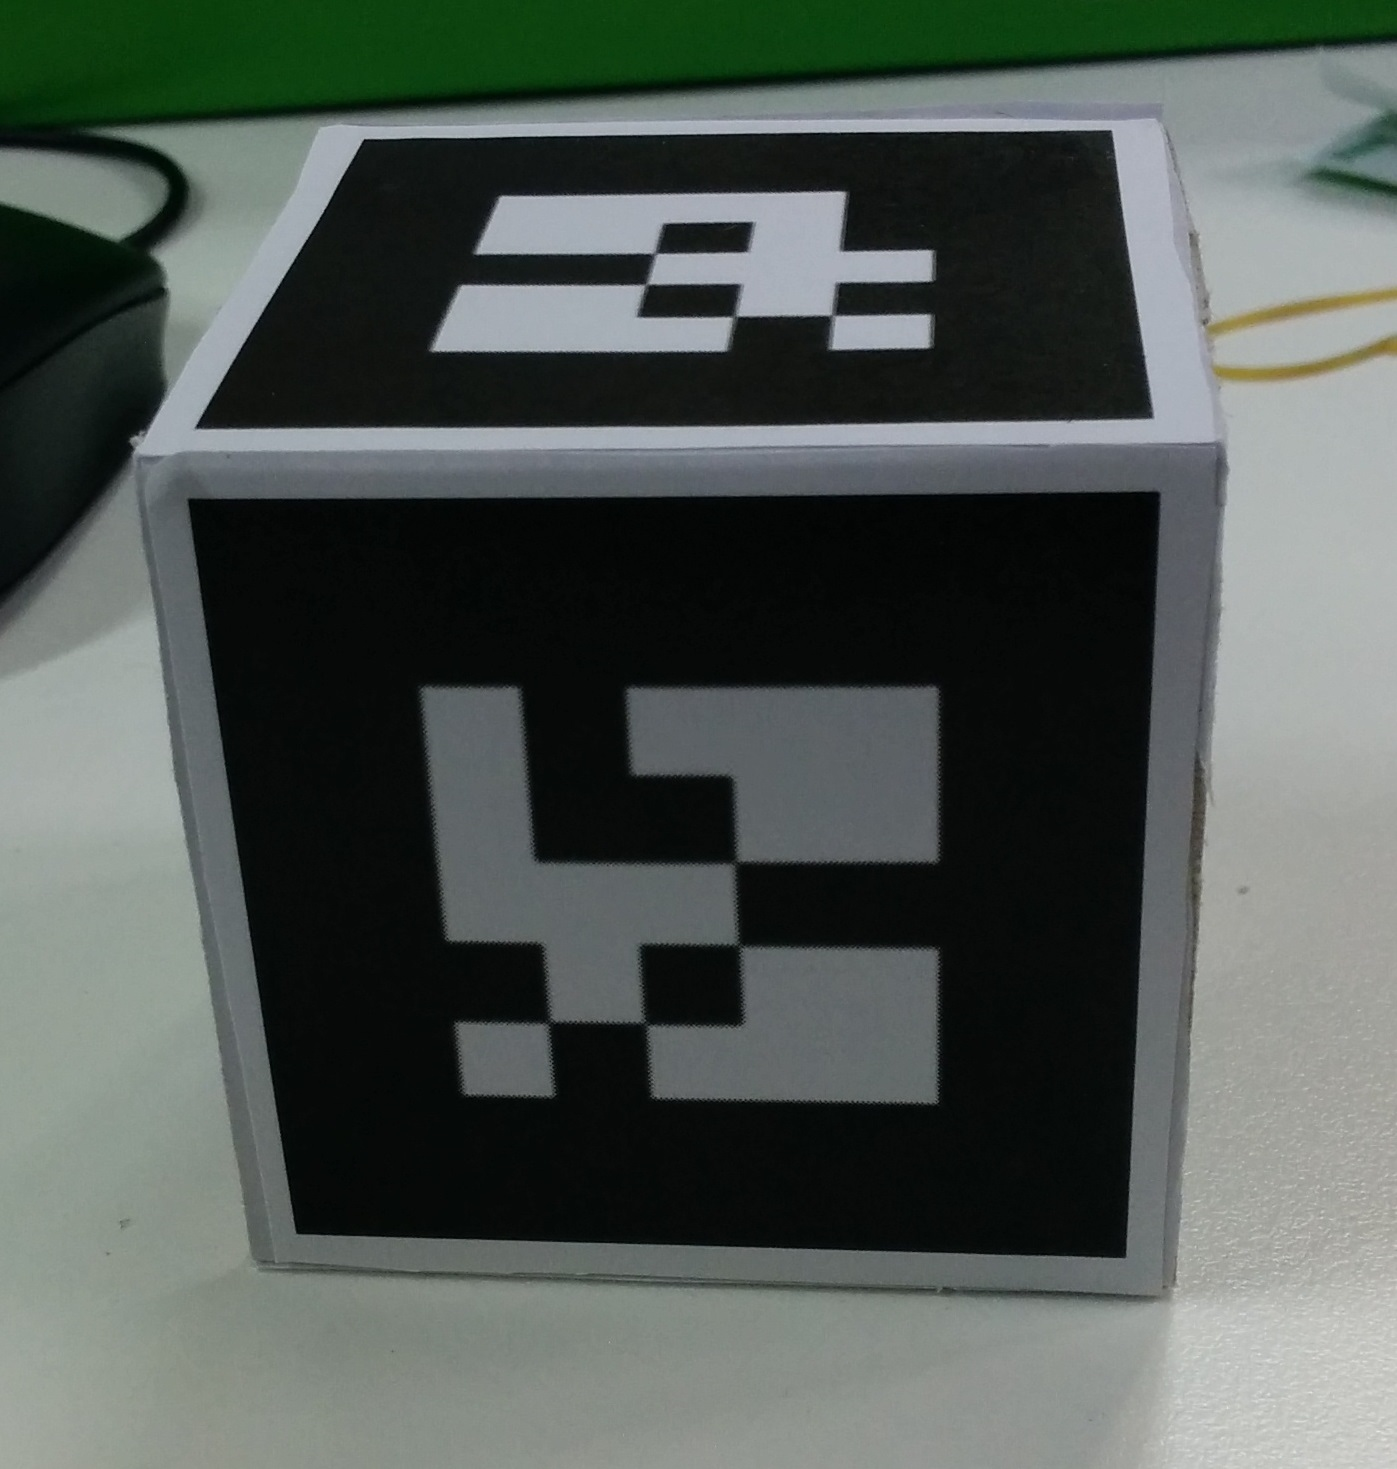
\includegraphics[width=0.8\textwidth]{pictures/marker_cube.jpg}
%           
%    \end{figure}										 
\end{itemize}   
& 
  \begin{itemize}
  \item Trying to evaluate BLORT, TrackerQt and Chilitags in Ubuntu in virtual machine ( will use some monocular camera supported by OpenCV to test). If the results are promising will try to setup in windows.
\end{itemize}  \\
\hline
  										 
  
  2015/03/04        & 
  \begin{itemize}
  \item Fixed the OpenGLSL errors in BLORT (GLSL Frag and Vert file errors). Both BLORT and TrackerQt requires GPU. Confirmed with Thomas Morwald (developer)
  \item Checked chilitags with webcam in ubuntu (14.04) environment. It is not as reliable as ALVAR toolkit. Also there are memory leaks.
  \item Ported robot\_description sample from Nao Simulator sdk 1.14 to sdk 2.1.2 ( for exporting urdf file of the robot model)
  \item Setup PWP3D tracking library (Need CUDA GPU)
  \item Naoqi setup in Ubuntu
  \item Setting up openrave environment (thinking of use it as a simulation environment. put both robot and human in openrave simulator - don't know if it is good idea. But will give it a try)
\end{itemize}   
  										 & - \\
  \hline
  
  2015/03/05         & 
  \begin{itemize}
  \item Experiment with Jean (Reflective marker tracking on subjects head. Captured video using kinect studio). Also checked the marker tracking by putting the marker on Nao robot's head and made a video (\url{http://youtu.be/VB0LHJM0dwI}). Marker tracking affected by lighting. 
  \item Setup ROS nao and openrave build.
  \item Investigated if VREP could be used as simulation environment ( It has a nao model but it is old. it has to be updated)
  \item Serial kinematic chain model for the case when Marker is put on Nao's head.  (has to be checked after implementation and experimentation)
\end{itemize}   
  & 
\\  										 \hline

  2015/03/06         & 
  \begin{itemize}
  \item Computing the pose of top of the marker cube when one or more of the markers are detected (if more than one quaternion slerp is used to find the best estimate)
  \item Setting up openrave
  \item Prepare Nao meshes and conversion of Urdf to dae ( wrote a simple ros node to do this)
\end{itemize}   
  & 
  \begin{itemize}
  										 \item Openrave build unsuccessful. 
  										 \item Dae conversion unsuccessful
  										 \end{itemize} \\
  										 \hline
  										 
	 2015/03/07         & 
  \begin{itemize}
  \item Kinematic model design and implement implement in Python-sympy ( for quick checking)
  \item Visited Mujin bot office (\url{www.mujin.co.jp}). They do some impressive work in the field of industrial robotics
\end{itemize}   
  & 
-  					\\					 \hline  	

2015/03/08         & 
  \begin{itemize}
  \item Continued with openrave setup
\end{itemize}   
  & 
-  					\\					 \hline  										 
  										   										 
    \end{longtable}
\end{center}

\newpage
\section{2015/03/09-2015/03/15}

\begin{center}
    \begin{longtable}{ | c | p{6cm} | p{5cm} |}
    \hline
    Date & Content & Problems/Remarks \\ 
    \endhead
    \hline    
     2015/03/09         & 
  \begin{itemize}
  \item Openrave setup complete
  \item Collada export using collada\_urdf exporter
\end{itemize}  
   & collada\_urdf exporter not working with Ubuntu 14.04 and ROS indigo. Have to try with ROS Hydro \\
\hline
  										 
 2015/03/10         & 
  \begin{itemize}
  \item Studied usage of VisualGestureBuilder tool. Tried generating simple hand wave gesture
  \item Made a sample application to test the generated gesture database
\end{itemize}   
& 
  \begin{itemize}
  \item With both Left and right hand gestures available, only one of them is detected properly. Debugging to understand the problem
\end{itemize}  \\
\hline
  										 
  
  2015/03/11        & 
  \begin{itemize}
  \item Fixed the bug in the gesture recognition sample. The sample video is uploaded at \url{http://youtu.be/7E8TgLbQ4a8}
  \item Kinect V2 setup guide documentation
  \item Nao Robot collada model export successful - Finally !!! ( Possible with ROS Hydro in Ubuntu 12.04 virtual machine)
\end{itemize}   
  										 & - \\
  \hline
  
  2015/03/12         & 
  \begin{itemize}
  \item Optimizing the 3d collada model of Nao
\end{itemize}   
  & 
\\  										 \hline

  2015/03/13         & 
  \begin{itemize}
  \item Investigated the possibility to use Protobuf as interprocess communication exchange format
  \item Minor changes to the Experimot
  \item Try openrave-2013 build
  \item Joint data acquisition of Nao robot when Tai-chi motion is performed.
\end{itemize}   
  & 
- \\
  										 \hline
  										 
	 2015/03/14         & 
  \begin{itemize}
  \item openrave-2013 build successful
  \item Protobuf build
  \item Decided to use Protobuf messages used in Gazebo to be used for the platform I am developing
\end{itemize}   
  & 
-  					\\					 \hline  	

2015/03/15         & 
  \begin{itemize}
  \item Created a custom marker cube for Nao pose detection ( Cube bought from - \url{http://www.amazon.co.jp/dp/B0049EVGC4/ref=pe_492632_159100282_TE_item} )
  \item Imported Gazebo messages from repository and wrote an automatic script to export the headers and source files from *.proto files.
  \item Tested the export script and static library creation
\end{itemize}   
  & 
-  					\\					 \hline  										 
  										   										 
    \end{longtable}
\end{center}

\newpage
\section{2015/03/16-2015/03/22}

\begin{center}
    \begin{longtable}{ | c | p{6cm} | p{5cm} |}
    \hline
    Date & Content & Problems/Remarks \\ 
    \endhead
    \hline    
     2015/03/16         & 
  \begin{itemize}
  \item Seminar: Symptoms of being alive and shared life at Keio University
  \begin{itemize}
	\item Talks on life, emerging new organisms, non-verbal communication in human robot interaction, life and turing machine, di-chronic study using coral atolls, human chimpanzee interaction, animals perception of life.	  
  \end{itemize}
  \item Observations relevant to my project
  \begin{itemize}
  	\item Using ethics to interact may give the impression that the thing is living. 
	\item The manner in which an agent/robot spends its idle time will have a greater impact on its liveliness.
  \end{itemize}
\end{itemize}  
- \\
\hline
  										 
 2015/03/17         & 
  \begin{itemize}
  \item The joint values of the tai chi pose of Nao collected last week is used to simulate the Nao robot in openrave environment - Successful!
  \item The video is uploaded at \url{http://youtu.be/aFECThEAivk}
\end{itemize}   
& 
  -  \\
\hline
  										 
  
  2015/03/18        & 
  \begin{itemize}
  \item Boost ASIO and ZMQ setup.
  \item Seminar
\end{itemize}   
  										 & - \\
  \hline
  
  2015/03/19         & 
  \begin{itemize}
  \item Created kinect Video playback tool (\url{http://youtu.be/vUdm8QeylP4})
  \item Boost ASIO and ZMQ client/server development
  \item Meeting
\end{itemize}   
  & 
\\  										 \hline

  2015/03/20         & 
  \begin{itemize}
  \item Successfully got protobuf and zeromq working together
  \item Tested the joint value simulation using client server architecture
  \item Also tried with the python publisher. Inter-process communication works as expected.
\end{itemize}   
  & 
- \\
  										 \hline
  																	 
  										   										 
    \end{longtable}
\end{center}

\newpage
\section{2015/03/23-2015/03/29}

\begin{center}
    \begin{longtable}{ | c | p{6cm} | p{5cm} |}
    \hline
    Date & Content & Problems/Remarks \\ 
    \endhead
    \hline    
     2015/03/23         & 
  \begin{itemize}
  \item Improved Kinect XEF File Playback tool (File Open, Display Body Index Frame etc.,)
  \item Auto generation of C\# classes from .proto files. Created the C\# library containing the generated messages
  \item Tested the IPC between the C\# application and OpenRave client application - Works perfectly!
  \item Kinect body information publication/subscription test
\end{itemize}  
   & Kinect Playback Tool - The way to read the skeleton information from the event stream is still unknown. Have to figure it out. \\
\hline
  										 
 2015/03/24         & 
  \begin{itemize}
  \item Kinect body information display in openrave environment alongside Nao robot. - Works well 
  \item Real time Nao robot simulation in OpenRave environment (\url{http://youtu.be/wUgRbslD6jk})
  \item Absolute localization based on markers - test started
\end{itemize}   
& 
  \begin{itemize}
  \item -
\end{itemize}  \\
\hline
  										 
  
  2015/03/25        & 
  \begin{itemize}
  \item Integration of localization module in the framework (experimot\_localization)
  \item Kinect Playback tool IR stream support added
\end{itemize}   
  										 & - \\
  \hline
  
  2015/03/26         & 
  \begin{itemize}
  \item Integration of localization module. Developed nao Marker frame forward kinematics module and tested against openrave forward kinematics.
\end{itemize}   
  & 
\\  										 \hline

  2015/03/27         & 
  \begin{itemize}
  \item Major refacoring of localization module
  \item Unit testing
  \item Localization IPC setup
\end{itemize}   
  & 
- \\
  										 \hline
  										 
	 2015/03/28         & 
  \begin{itemize}
  \item Bug fixes
  \item Complete communication flow test (Localization, Robot-interface, Skeleton-tracking, Simulator)
\end{itemize}   
  & 
\begin{itemize}
\item Need to fine tune localization. Position looks good. Orientation is a concern ( TODO Item : Modify the way in which the torso frame is computed. )
\item Coordinate frames has to be synchronized.
\end{itemize}			\\					 \hline  	

2015/03/29         & 
  \begin{itemize}
  \item Quartz scheduler - Feasibility study (Looks promising)
\end{itemize}   
  & 
-  					\\					 \hline  										 
  										   										 
    \end{longtable}
\end{center}

\newpage
\section{2015/03/30-2015/04/05}

\begin{center}
    \begin{longtable}{ | c | p{6cm} | p{5cm} |}
    \hline
    Date & Content & Problems/Remarks \\ 
    \endhead
    \hline    
     2015/03/30         & 
  \begin{itemize}
  \item Nao localization test. Fixed the torso frame calculation bug. 
\end{itemize}  
   & The pose computation is still sometimes strange. The frames of reference are not perfectly synchronized. Need more test. \\
\hline
  										 
 2015/03/31         & 
  \begin{itemize}
  \item Fixed bugs in the Nao pose estimation.
  \item Added the color stream support in the kinect playback tool.
  \item Investigation on how to extract skeleton data from raw buffer in XEF file
\end{itemize}   
& 
  \begin{itemize}
  \item The raw format used by Microsoft for color stream was Yuy2 ( 4 bytes for 2 pixels). The conversion from Yuy2 to RGB was implemented in Kinect Playback tool
  \item The skeleton buffer was 6288 bytes. I tried decoding the skeleton values from the byte stream. Still cannot figure out how the data structure is aligned while serializing.
\end{itemize}  \\
\hline
  										 
  
  2015/04/01        & 
  \begin{itemize}
  \item Fixed Experimot studio startup problem.
  \item Scheduler design. Written core classes that will compose the Context of the scheduler.
  \end{itemize}   
  										 & - \\
  \hline
  
  2015/04/02         & 
  \begin{itemize}
  \item Schedule core classes design
  \item Localization reference frame problem debugging
\end{itemize}   
  & 
\\  										 \hline

  2015/04/03         & 
  \begin{itemize}
  \item Localization reference frame problem fix
  \item Testing
\end{itemize}   
  & 
  -
\\
  										 \hline
  										 
	 2015/04/04         & 
  \begin{itemize}
  \item Bug fixes in the localization
\end{itemize}   
  & 
\begin{itemize}
  \item The camera frame considered by ALVAR was (x-right, y-down and z-forward). However for KINECT it was (x-right, y-up and z-forward). So basically I had to invert the y-axis position values after computing the Torso pose.
  \item \emph{TODO}: Weighted pose estimation depending on the marker detection confidence.
\end{itemize}  		\\					 \hline  	

										 
  										   								 
    \end{longtable}
\end{center}

\newpage
\section{2015/04/06-2015/04/12}

\begin{center}
    \begin{longtable}{ | c | p{6cm} | p{5cm} |}
    \hline
    Date & Content & Problems/Remarks \\ 
    \endhead
    \hline    
     2015/04/06         & 
  \begin{itemize}
  \item Lab meeting
  \item Application bootstrapper - Modified XML schema to support node parameters. In the process of supplying the node parameters as a command line arguments to the individual nodes during startup.
\end{itemize}  
   & - \\
\hline
  										 
 2015/04/07         & 
  \begin{itemize}
  \item Application bootstrapper support - Extended the xml config file to support global and local parameters. global Parameter overriding, support the new configuration information in the individual nodes. 
  \item Testing the supported nodes. 
\end{itemize}   
& 
 \\
\hline
  										 
  
  2015/04/08        & 
  \begin{itemize}
  \item Node startup enable/disable support
  \item Integration of Gesture recognition and Skeleton tracking and supported start up of this node from configuration information.
  \item Application context information management support. Auto subscription of all the published messages. Under test
  \end{itemize}   
  										 & - \\
  \hline
  
  2015/04/09         & 
  \begin{itemize}
  \item Migration from clrzmq to NetMQ .NET library for ZeroMQ
  \item Parameter server and Context synchronization from all publishing nodes - Multi-threading support
  \item UI update of current pose from the context
\end{itemize}   
  & 
\\  										 \hline

  2015/04/10         & 
  \begin{itemize}
  \item Tried serializing the kinect body to cross check with the raw buffer size
  \item Kalman filter implementation started
  \item Fixed bugs in the localization module and testing
\end{itemize}   
  & 
  - Walking on the floor mat was not good. So will test once again on the room 452 next week
\\
  										 \hline
  										 
	 2015/04/11         & 
  \begin{itemize}
  \item Target Drives Means (TDM) Framework client python script development - To make the localization data available to the TDM framework
\end{itemize}   
  & 
		\\					 \hline  	

	 2015/04/12         & 
  \begin{itemize}
  \item Target Drives Means (TDM) Framework client python script development \& Testing - Works fine
  \item Will organize a meeting with Mr.Vincent Berenz next week and prepare for the initial integration test for the scenario of Nao robot walking to and fro between two locations.
\end{itemize}   
  & 
		\\					 \hline  	
										 
  										   								 
    \end{longtable}
\end{center}

\newpage
\section{2015/04/13-2015/04/19}

\begin{center}
    \begin{longtable}{ | c | p{6cm} | p{5cm} |}
    \hline
    Date & Content & Problems/Remarks \\ 
    \endhead
    \hline    
     2015/04/13         & 
  \begin{itemize}
  \item Lab meeting
  \item Python client preparation for Mr.Vincent Berenz to access localization information from my platform
  \item Bug Fix: Refreshing the simulation window when no Kinect body is detected
  \item In order to enhance the pose estimate, I plan to consider the depth information of the detected markers as well. To do this, I started integrating the PCL Grabber with Localization module.
\end{itemize}  
   & - \\
\hline
  										 
 2015/04/14         & 
  \begin{itemize}
  \item Made a python client sample plotting the pose of the robot on the plane using matplotlib
  \item Meeting with Mr. Vincent Berenz about the TDM framework. We agree d to develop a description of the world to communicate information between Experimot and TDM
  \item Continue implementation of Marker pose improvement taking into account of the kinect information.
  \item Median filter implementation
\end{itemize}   
& 
 \\
\hline
  										 
  
  2015/04/15        & 
  \begin{itemize}
  \item Kinect data integration for improved pose estimation
  \end{itemize}   
  										 & 
\begin{itemize}
  \item Point cloud organization caused lot of issues and creating problems by crashing the application. Found the source causing the problem and fixed the issue. However the Pose estimation using kinect is still not successful.
  \end{itemize}  
  										 \\
  \hline
  
  2015/04/16         & 
  \begin{itemize}
  \item Modified the point cloud generation using MapColorFrameToCameraSpace method of coordinate mapper. The Pose estimation is not stable and sometime the depth information is noisy and it give INFINITY for the depth value which crashes the localization module
  \item Started with the presentation
  \item Tried three.js to be used as the 3D viewer of the web site (trying the possibility of providing the web based monitor for human robot interaction)
\end{itemize}   
  & 
\\  										 \hline

  2015/04/17         & 
  \begin{itemize}
  \item Three.js robot loading verified. Refactoring the project structure
  \item Motion/Behavior modules registration mechanism implementation
  \item Made sample python script for calling the behavior installed in the robot
  \item Python node parameter retrieval support - ongoing
\end{itemize}   
  & 
  - 
\\
  										 \hline
  										 
	 2015/04/18         & 
  \begin{itemize}
  \item Target Drives Means (TDM) Framework client python script development - To make the localization data available to the TDM framework
\end{itemize}   
  & 
		\\					 \hline  	

	 2015/04/19         & 
  \begin{itemize}
  \item Target Drives Means (TDM) Framework client python script development \& Testing - Works fine
  \item Will organize a meeting with Mr.Vincent Berenz next week and prepare for the initial integration test for the scenario of Nao robot walking to and fro between two locations.
\end{itemize}   
  & 
		\\					 \hline  	
										 
  										   								 
    \end{longtable}
\end{center}

\end{document}